%%%%%%%%%%%%%%%%%%%%%%%%%%%%%%%%%%%%%%%%%
% The Legrand Orange Book
% LaTeX Template
% Version 2.4 (26/09/2018)
%
% This template was downloaded from:
% http://www.LaTeXTemplates.com
%
% Original author:
% Mathias Legrand (legrand.mathias@gmail.com) with modifications by:
% Vel (vel@latextemplates.com)
%
% License:
% CC BY-NC-SA 3.0 (http://creativecommons.org/licenses/by-nc-sa/3.0/)
%
% Compiling this template:
% This template uses biber for its bibliography and makeindex for its index.
% When you first open the template, compile it from the command line with the 
% commands below to make sure your LaTeX distribution is configured correctly:
%
% 1) pdflatex main
% 2) makeindex main.idx -s StyleInd.ist
% 3) biber main
% 4) pdflatex main x 2
%
% After this, when you wish to update the bibliography/index use the appropriate
% command above and make sure to compile with pdflatex several times 
% afterwards to propagate your changes to the document.
%
% This template also uses a number of packages which may need to be
% updated to the newest versions for the template to compile. It is strongly
% recommended you update your LaTeX distribution if you have any
% compilation errors.
%
% Important note:
% Chapter heading images should have a 2:1 width:height ratio,
% e.g. 920px width and 460px height.
%
%%%%%%%%%%%%%%%%%%%%%%%%%%%%%%%%%%%%%%%%%

%----------------------------------------------------------------------------------------
%	PACKAGES AND OTHER DOCUMENT CONFIGURATIONS
%----------------------------------------------------------------------------------------

\documentclass[11pt,fleqn]{book} % Default font size and left-justified equations

%%%%%%%%%%%%%%%%%%%%%%%%%%%%%%%%%%%%%%%%%
% The Legrand Orange Book
% Structural Definitions File
% Version 2.1 (26/09/2018)
%
% Original author:
% Mathias Legrand (legrand.mathias@gmail.com) with modifications by:
% Vel (vel@latextemplates.com)
% 
% This file was downloaded from:
% http://www.LaTeXTemplates.com
%
% License:
% CC BY-NC-SA 3.0 (http://creativecommons.org/licenses/by-nc-sa/3.0/)
%
%%%%%%%%%%%%%%%%%%%%%%%%%%%%%%%%%%%%%%%%%

%----------------------------------------------------------------------------------------
%	VARIOUS REQUIRED PACKAGES AND CONFIGURATIONS
%----------------------------------------------------------------------------------------

\usepackage{graphicx} % Required for including pictures
\graphicspath{{Pictures/}} % Specifies the directory where pictures are stored

\usepackage{lipsum} % Inserts dummy text

\usepackage{tikz} % Required for drawing custom shapes

\usepackage[english]{babel} % English language/hyphenation

\usepackage{enumitem} % Customize lists
\setlist{nolistsep} % Reduce spacing between bullet points and numbered lists

\usepackage{booktabs} % Required for nicer horizontal rules in tables

\usepackage{xcolor} % Required for specifying colors by name
\definecolor{ocre}{RGB}{40,122,255} % Define the orange color used for highlighting throughout the book

%----------------------------------------------------------------------------------------
%	MARGINS
%----------------------------------------------------------------------------------------

\usepackage{geometry} % Required for adjusting page dimensions and margins

\geometry{
	paper=a4paper, % Paper size, change to letterpaper for US letter size
	top=3cm, % Top margin
	bottom=3cm, % Bottom margin
	left=3cm, % Left margin
	right=3cm, % Right margin
	headheight=14pt, % Header height
	footskip=1.4cm, % Space from the bottom margin to the baseline of the footer
	headsep=10pt, % Space from the top margin to the baseline of the header
	%showframe, % Uncomment to show how the type block is set on the page
}

%----------------------------------------------------------------------------------------
%	FONTS
%----------------------------------------------------------------------------------------

\usepackage{avant} % Use the Avantgarde font for headings
%\usepackage{times} % Use the Times font for headings
\usepackage{mathptmx} % Use the Adobe Times Roman as the default text font together with math symbols from the Sym­bol, Chancery and Com­puter Modern fonts

\usepackage{microtype} % Slightly tweak font spacing for aesthetics
\usepackage[utf8]{inputenc} % Required for including letters with accents
\usepackage[T1]{fontenc} % Use 8-bit encoding that has 256 glyphs

%----------------------------------------------------------------------------------------
%	BIBLIOGRAPHY AND INDEX
%----------------------------------------------------------------------------------------

\usepackage[style=numeric,citestyle=numeric,sorting=nyt,sortcites=true,autopunct=true,babel=hyphen,hyperref=true,abbreviate=false,backref=true,backend=biber]{biblatex}
\addbibresource{bibliography.bib} % BibTeX bibliography file
\defbibheading{bibempty}{}

\usepackage{calc} % For simpler calculation - used for spacing the index letter headings correctly
\usepackage{makeidx} % Required to make an index
\makeindex % Tells LaTeX to create the files required for indexing

%----------------------------------------------------------------------------------------
%	MAIN TABLE OF CONTENTS
%----------------------------------------------------------------------------------------

\usepackage{titletoc} % Required for manipulating the table of contents

\contentsmargin{0cm} % Removes the default margin

% Part text styling (this is mostly taken care of in the PART HEADINGS section of this file)
\titlecontents{part}
	[0cm] % Left indentation
	{\addvspace{20pt}\bfseries} % Spacing and font options for parts
	{}
	{}
	{}

% Chapter text styling
\titlecontents{chapter}
	[1.25cm] % Left indentation
	{\addvspace{12pt}\large\sffamily\bfseries} % Spacing and font options for chapters
	{\color{ocre!60}\contentslabel[\Large\thecontentslabel]{1.25cm}\color{ocre}} % Formatting of numbered sections of this type
	{\color{ocre}} % Formatting of numberless sections of this type
	{\color{ocre!60}\normalsize\;\titlerule*[.5pc]{.}\;\thecontentspage} % Formatting of the filler to the right of the heading and the page number

% Section text styling
\titlecontents{section}
	[1.25cm] % Left indentation
	{\addvspace{3pt}\sffamily\bfseries} % Spacing and font options for sections
	{\contentslabel[\thecontentslabel]{1.25cm}} % Formatting of numbered sections of this type
	{} % Formatting of numberless sections of this type
	{\hfill\color{black}\thecontentspage} % Formatting of the filler to the right of the heading and the page number

% Subsection text styling
\titlecontents{subsection}
	[1.25cm] % Left indentation
	{\addvspace{1pt}\sffamily\small} % Spacing and font options for subsections
	{\contentslabel[\thecontentslabel]{1.25cm}} % Formatting of numbered sections of this type
	{} % Formatting of numberless sections of this type
	{\ \titlerule*[.5pc]{.}\;\thecontentspage} % Formatting of the filler to the right of the heading and the page number

% Figure text styling
\titlecontents{figure}
	[1.25cm] % Left indentation
	{\addvspace{1pt}\sffamily\small} % Spacing and font options for figures
	{\thecontentslabel\hspace*{1em}} % Formatting of numbered sections of this type
	{} % Formatting of numberless sections of this type
	{\ \titlerule*[.5pc]{.}\;\thecontentspage} % Formatting of the filler to the right of the heading and the page number

% Table text styling
\titlecontents{table}
	[1.25cm] % Left indentation
	{\addvspace{1pt}\sffamily\small} % Spacing and font options for tables
	{\thecontentslabel\hspace*{1em}} % Formatting of numbered sections of this type
	{} % Formatting of numberless sections of this type
	{\ \titlerule*[.5pc]{.}\;\thecontentspage} % Formatting of the filler to the right of the heading and the page number

%----------------------------------------------------------------------------------------
%	MINI TABLE OF CONTENTS IN PART HEADS
%----------------------------------------------------------------------------------------

% Chapter text styling
\titlecontents{lchapter}
	[0em] % Left indentation
	{\addvspace{15pt}\large\sffamily\bfseries} % Spacing and font options for chapters
	{\color{ocre}\contentslabel[\Large\thecontentslabel]{1.25cm}\color{ocre}} % Chapter number
	{}  
	{\color{ocre}\normalsize\sffamily\bfseries\;\titlerule*[.5pc]{.}\;\thecontentspage} % Page number

% Section text styling
\titlecontents{lsection}
	[0em] % Left indentation
	{\sffamily\small} % Spacing and font options for sections
	{\contentslabel[\thecontentslabel]{1.25cm}} % Section number
	{}
	{}

% Subsection text styling (note these aren't shown by default, display them by searchings this file for tocdepth and reading the commented text)
\titlecontents{lsubsection}
	[.5em] % Left indentation
	{\sffamily\footnotesize} % Spacing and font options for subsections
	{\contentslabel[\thecontentslabel]{1.25cm}}
	{}
	{}

%----------------------------------------------------------------------------------------
%	HEADERS AND FOOTERS
%----------------------------------------------------------------------------------------

\usepackage{fancyhdr} % Required for header and footer configuration

\pagestyle{fancy} % Enable the custom headers and footers

\renewcommand{\chaptermark}[1]{\markboth{\sffamily\normalsize\bfseries\chaptername\ \thechapter.\ #1}{}} % Styling for the current chapter in the header
\renewcommand{\sectionmark}[1]{\markright{\sffamily\normalsize\thesection\hspace{5pt}#1}{}} % Styling for the current section in the header

\fancyhf{} % Clear default headers and footers
\fancyhead[LE,RO]{\sffamily\normalsize\thepage} % Styling for the page number in the header
\fancyhead[LO]{\rightmark} % Print the nearest section name on the left side of odd pages
\fancyhead[RE]{\leftmark} % Print the current chapter name on the right side of even pages
%\fancyfoot[C]{\thepage} % Uncomment to include a footer

\renewcommand{\headrulewidth}{0.5pt} % Thickness of the rule under the header

\fancypagestyle{plain}{% Style for when a plain pagestyle is specified
	\fancyhead{}\renewcommand{\headrulewidth}{0pt}%
}

% Removes the header from odd empty pages at the end of chapters
\makeatletter
\renewcommand{\cleardoublepage}{
\clearpage\ifodd\c@page\else
\hbox{}
\vspace*{\fill}
\thispagestyle{empty}
\newpage
\fi}

%----------------------------------------------------------------------------------------
%	THEOREM STYLES
%----------------------------------------------------------------------------------------

\usepackage{amsmath,amsfonts,amssymb,amsthm} % For math equations, theorems, symbols, etc

\newcommand{\intoo}[2]{\mathopen{]}#1\,;#2\mathclose{[}}
\newcommand{\ud}{\mathop{\mathrm{{}d}}\mathopen{}}
\newcommand{\intff}[2]{\mathopen{[}#1\,;#2\mathclose{]}}
\renewcommand{\qedsymbol}{$\blacksquare$}
\newtheorem{notation}{Notation}[chapter]

% Boxed/framed environments
\newtheoremstyle{ocrenumbox}% Theorem style name
{0pt}% Space above
{0pt}% Space below
{\normalfont}% Body font
{}% Indent amount
{\small\bf\sffamily\color{ocre}}% Theorem head font
{\;}% Punctuation after theorem head
{0.25em}% Space after theorem head
{\small\sffamily\color{ocre}\thmname{#1}\nobreakspace\thmnumber{\@ifnotempty{#1}{}\@upn{#2}}% Theorem text (e.g. Theorem 2.1)
\thmnote{\nobreakspace\the\thm@notefont\sffamily\bfseries\color{black}---\nobreakspace#3.}} % Optional theorem note

\newtheoremstyle{blacknumex}% Theorem style name
{5pt}% Space above
{5pt}% Space below
{\normalfont}% Body font
{} % Indent amount
{\small\bf\sffamily}% Theorem head font
{\;}% Punctuation after theorem head
{0.25em}% Space after theorem head
{\small\sffamily{\tiny\ensuremath{\blacksquare}}\nobreakspace\thmname{#1}\nobreakspace\thmnumber{\@ifnotempty{#1}{}\@upn{#2}}% Theorem text (e.g. Theorem 2.1)
\thmnote{\nobreakspace\the\thm@notefont\sffamily\bfseries---\nobreakspace#3.}}% Optional theorem note

\newtheoremstyle{blacknumbox} % Theorem style name
{0pt}% Space above
{0pt}% Space below
{\normalfont}% Body font
{}% Indent amount
{\small\bf\sffamily}% Theorem head font
{\;}% Punctuation after theorem head
{0.25em}% Space after theorem head
{\small\sffamily\thmname{#1}\nobreakspace\thmnumber{\@ifnotempty{#1}{}\@upn{#2}}% Theorem text (e.g. Theorem 2.1)
\thmnote{\nobreakspace\the\thm@notefont\sffamily\bfseries---\nobreakspace#3.}}% Optional theorem note

% Non-boxed/non-framed environments
\newtheoremstyle{ocrenum}% Theorem style name
{5pt}% Space above
{5pt}% Space below
{\normalfont}% Body font
{}% Indent amount
{\small\bf\sffamily\color{ocre}}% Theorem head font
{\;}% Punctuation after theorem head
{0.25em}% Space after theorem head
{\small\sffamily\color{ocre}\thmname{#1}\nobreakspace\thmnumber{\@ifnotempty{#1}{}\@upn{#2}}% Theorem text (e.g. Theorem 2.1)
\thmnote{\nobreakspace\the\thm@notefont\sffamily\bfseries\color{black}---\nobreakspace#3.}} % Optional theorem note
\makeatother

% Defines the theorem text style for each type of theorem to one of the three styles above
\newcounter{dummy} 
\numberwithin{dummy}{section}
\theoremstyle{ocrenumbox}
\newtheorem{theoremeT}[dummy]{Theorem}
\newtheorem{problem}{Problem}[chapter]
\newtheorem{exerciseT}{Exercise}[chapter]
\theoremstyle{blacknumex}
\newtheorem{exampleT}{Example}[chapter]
\theoremstyle{blacknumbox}
\newtheorem{vocabulary}{Vocabulary}[chapter]
\newtheorem{definitionT}{Definition}[section]
\newtheorem{corollaryT}[dummy]{Corollary}
\theoremstyle{ocrenum}
\newtheorem{proposition}[dummy]{Proposition}

%----------------------------------------------------------------------------------------
%	DEFINITION OF COLORED BOXES
%----------------------------------------------------------------------------------------

\RequirePackage[framemethod=default]{mdframed} % Required for creating the theorem, definition, exercise and corollary boxes

% Theorem box
\newmdenv[skipabove=7pt,
skipbelow=7pt,
backgroundcolor=black!5,
linecolor=ocre,
innerleftmargin=5pt,
innerrightmargin=5pt,
innertopmargin=5pt,
leftmargin=0cm,
rightmargin=0cm,
innerbottommargin=5pt]{tBox}

% Exercise box	  
\newmdenv[skipabove=7pt,
skipbelow=7pt,
rightline=false,
leftline=true,
topline=false,
bottomline=false,
backgroundcolor=ocre!10,
linecolor=ocre,
innerleftmargin=5pt,
innerrightmargin=5pt,
innertopmargin=5pt,
innerbottommargin=5pt,
leftmargin=0cm,
rightmargin=0cm,
linewidth=4pt]{eBox}	

% Definition box
\newmdenv[skipabove=7pt,
skipbelow=7pt,
rightline=false,
leftline=true,
topline=false,
bottomline=false,
linecolor=ocre,
innerleftmargin=5pt,
innerrightmargin=5pt,
innertopmargin=0pt,
leftmargin=0cm,
rightmargin=0cm,
linewidth=4pt,
innerbottommargin=0pt]{dBox}	

% Corollary box
\newmdenv[skipabove=7pt,
skipbelow=7pt,
rightline=false,
leftline=true,
topline=false,
bottomline=false,
linecolor=gray,
backgroundcolor=black!5,
innerleftmargin=5pt,
innerrightmargin=5pt,
innertopmargin=5pt,
leftmargin=0cm,
rightmargin=0cm,
linewidth=4pt,
innerbottommargin=5pt]{cBox}

% Creates an environment for each type of theorem and assigns it a theorem text style from the "Theorem Styles" section above and a colored box from above
\newenvironment{theorem}{\begin{tBox}\begin{theoremeT}}{\end{theoremeT}\end{tBox}}
\newenvironment{exercise}{\begin{eBox}\begin{exerciseT}}{\hfill{\color{ocre}\tiny\ensuremath{\blacksquare}}\end{exerciseT}\end{eBox}}				  
\newenvironment{definition}{\begin{dBox}\begin{definitionT}}{\end{definitionT}\end{dBox}}	
\newenvironment{example}{\begin{exampleT}}{\hfill{\tiny\ensuremath{\blacksquare}}\end{exampleT}}		
\newenvironment{corollary}{\begin{cBox}\begin{corollaryT}}{\end{corollaryT}\end{cBox}}	

%----------------------------------------------------------------------------------------
%	REMARK ENVIRONMENT
%----------------------------------------------------------------------------------------

\newenvironment{remark}{\par\vspace{10pt}\small % Vertical white space above the remark and smaller font size
\begin{list}{}{
\leftmargin=35pt % Indentation on the left
\rightmargin=25pt}\item\ignorespaces % Indentation on the right
\makebox[-2.5pt]{\begin{tikzpicture}[overlay]
\node[draw=ocre!60,line width=1pt,circle,fill=ocre!25,font=\sffamily\bfseries,inner sep=2pt,outer sep=0pt] at (-15pt,0pt){\textcolor{ocre}{R}};\end{tikzpicture}} % Orange R in a circle
\advance\baselineskip -1pt}{\end{list}\vskip5pt} % Tighter line spacing and white space after remark

%----------------------------------------------------------------------------------------
%	SECTION NUMBERING IN THE MARGIN
%----------------------------------------------------------------------------------------

\makeatletter
\renewcommand{\@seccntformat}[1]{\llap{\textcolor{ocre}{\csname the#1\endcsname}\hspace{1em}}}                    
\renewcommand{\section}{\@startsection{section}{1}{\z@}
{-4ex \@plus -1ex \@minus -.4ex}
{1ex \@plus.2ex }
{\normalfont\large\sffamily\bfseries}}
\renewcommand{\subsection}{\@startsection {subsection}{2}{\z@}
{-3ex \@plus -0.1ex \@minus -.4ex}
{0.5ex \@plus.2ex }
{\normalfont\sffamily\bfseries}}
\renewcommand{\subsubsection}{\@startsection {subsubsection}{3}{\z@}
{-2ex \@plus -0.1ex \@minus -.2ex}
{.2ex \@plus.2ex }
{\normalfont\small\sffamily\bfseries}}                        
\renewcommand\paragraph{\@startsection{paragraph}{4}{\z@}
{-2ex \@plus-.2ex \@minus .2ex}
{.1ex}
{\normalfont\small\sffamily\bfseries}}

%----------------------------------------------------------------------------------------
%	PART HEADINGS
%----------------------------------------------------------------------------------------

% Numbered part in the table of contents
\newcommand{\@mypartnumtocformat}[2]{%
	\setlength\fboxsep{0pt}%
	\noindent\colorbox{ocre!20}{\strut\parbox[c][.7cm]{\ecart}{\color{ocre!70}\Large\sffamily\bfseries\centering#1}}\hskip\esp\colorbox{ocre!40}{\strut\parbox[c][.7cm]{\linewidth-\ecart-\esp}{\Large\sffamily\centering#2}}%
}

% Unnumbered part in the table of contents
\newcommand{\@myparttocformat}[1]{%
	\setlength\fboxsep{0pt}%
	\noindent\colorbox{ocre!40}{\strut\parbox[c][.7cm]{\linewidth}{\Large\sffamily\centering#1}}%
}

\newlength\esp
\setlength\esp{4pt}
\newlength\ecart
\setlength\ecart{1.2cm-\esp}
\newcommand{\thepartimage}{}%
\newcommand{\partimage}[1]{\renewcommand{\thepartimage}{#1}}%
\def\@part[#1]#2{%
\ifnum \c@secnumdepth >-2\relax%
\refstepcounter{part}%
\addcontentsline{toc}{part}{\texorpdfstring{\protect\@mypartnumtocformat{\thepart}{#1}}{\partname~\thepart\ ---\ #1}}
\else%
\addcontentsline{toc}{part}{\texorpdfstring{\protect\@myparttocformat{#1}}{#1}}%
\fi%
\startcontents%
\markboth{}{}%
{\thispagestyle{empty}%
\begin{tikzpicture}[remember picture,overlay]%
\node at (current page.north west){\begin{tikzpicture}[remember picture,overlay]%	
\fill[ocre!20](0cm,0cm) rectangle (\paperwidth,-\paperheight);
\node[anchor=north] at (4cm,-3.25cm){\color{ocre!40}\fontsize{220}{100}\sffamily\bfseries\thepart}; 
\node[anchor=south east] at (\paperwidth-1cm,-\paperheight+1cm){\parbox[t][][t]{8.5cm}{
\printcontents{l}{0}{\setcounter{tocdepth}{1}}% The depth to which the Part mini table of contents displays headings; 0 for chapters only, 1 for chapters and sections and 2 for chapters, sections and subsections
}};
\node[anchor=north east] at (\paperwidth-1.5cm,-3.25cm){\parbox[t][][t]{15cm}{\strut\raggedleft\color{white}\fontsize{30}{30}\sffamily\bfseries#2}};
\end{tikzpicture}};
\end{tikzpicture}}%
\@endpart}
\def\@spart#1{%
\startcontents%
\phantomsection
{\thispagestyle{empty}%
\begin{tikzpicture}[remember picture,overlay]%
\node at (current page.north west){\begin{tikzpicture}[remember picture,overlay]%	
\fill[ocre!20](0cm,0cm) rectangle (\paperwidth,-\paperheight);
\node[anchor=north east] at (\paperwidth-1.5cm,-3.25cm){\parbox[t][][t]{15cm}{\strut\raggedleft\color{white}\fontsize{30}{30}\sffamily\bfseries#1}};
\end{tikzpicture}};
\end{tikzpicture}}
\addcontentsline{toc}{part}{\texorpdfstring{%
\setlength\fboxsep{0pt}%
\noindent\protect\colorbox{ocre!40}{\strut\protect\parbox[c][.7cm]{\linewidth}{\Large\sffamily\protect\centering #1\quad\mbox{}}}}{#1}}%
\@endpart}
\def\@endpart{\vfil\newpage
\if@twoside
\if@openright
\null
\thispagestyle{empty}%
\newpage
\fi
\fi
\if@tempswa
\twocolumn
\fi}

%----------------------------------------------------------------------------------------
%	CHAPTER HEADINGS
%----------------------------------------------------------------------------------------

% A switch to conditionally include a picture, implemented by Christian Hupfer
\newif\ifusechapterimage
\usechapterimagetrue
\newcommand{\thechapterimage}{}%
\newcommand{\chapterimage}[1]{\ifusechapterimage\renewcommand{\thechapterimage}{#1}\fi}%
\newcommand{\autodot}{.}
\def\@makechapterhead#1{%
{\parindent \z@ \raggedright \normalfont
\ifnum \c@secnumdepth >\m@ne
\if@mainmatter
\begin{tikzpicture}[remember picture,overlay]
\node at (current page.north west)
{\begin{tikzpicture}[remember picture,overlay]
\node[anchor=north west,inner sep=0pt] at (0,0) {\ifusechapterimage\includegraphics[width=\paperwidth]{\thechapterimage}\fi};
\draw[anchor=west] (\Gm@lmargin,-9cm) node [line width=2pt,rounded corners=15pt,draw=ocre,fill=white,fill opacity=0.5,inner sep=15pt]{\strut\makebox[22cm]{}};
\draw[anchor=west] (\Gm@lmargin+.3cm,-9cm) node {\huge\sffamily\bfseries\color{black}\thechapter\autodot~#1\strut};
\end{tikzpicture}};
\end{tikzpicture}
\else
\begin{tikzpicture}[remember picture,overlay]
\node at (current page.north west)
{\begin{tikzpicture}[remember picture,overlay]
\node[anchor=north west,inner sep=0pt] at (0,0) {\ifusechapterimage\includegraphics[width=\paperwidth]{\thechapterimage}\fi};
\draw[anchor=west] (\Gm@lmargin,-9cm) node [line width=2pt,rounded corners=15pt,draw=ocre,fill=white,fill opacity=0.5,inner sep=15pt]{\strut\makebox[22cm]{}};
\draw[anchor=west] (\Gm@lmargin+.3cm,-9cm) node {\huge\sffamily\bfseries\color{black}#1\strut};
\end{tikzpicture}};
\end{tikzpicture}
\fi\fi\par\vspace*{270\p@}}}

%-------------------------------------------

\def\@makeschapterhead#1{%
\begin{tikzpicture}[remember picture,overlay]
\node at (current page.north west)
{\begin{tikzpicture}[remember picture,overlay]
\node[anchor=north west,inner sep=0pt] at (0,0) {\ifusechapterimage\includegraphics[width=\paperwidth]{\thechapterimage}\fi};
\draw[anchor=west] (\Gm@lmargin,-9cm) node [line width=2pt,rounded corners=15pt,draw=ocre,fill=white,fill opacity=0.5,inner sep=15pt]{\strut\makebox[22cm]{}};
\draw[anchor=west] (\Gm@lmargin+.3cm,-9cm) node {\huge\sffamily\bfseries\color{black}#1\strut};
\end{tikzpicture}};
\end{tikzpicture}
\par\vspace*{270\p@}}
\makeatother

%----------------------------------------------------------------------------------------
%	LINKS
%----------------------------------------------------------------------------------------

\usepackage{hyperref}
\hypersetup{hidelinks,backref=true,pagebackref=true,hyperindex=true,colorlinks=false,breaklinks=true,urlcolor=ocre,bookmarks=true,bookmarksopen=false}

\usepackage{bookmark}
\bookmarksetup{
open,
numbered,
addtohook={%
\ifnum\bookmarkget{level}=0 % chapter
\bookmarksetup{bold}%
\fi
\ifnum\bookmarkget{level}=-1 % part
\bookmarksetup{color=ocre,bold}%
\fi
}
}
 % Insert the commands.tex file which contains the majority of the structure behind the template

%\hypersetup{pdftitle={Title},pdfauthor={Author}} % Uncomment and fill out to include PDF metadata for the author and title of the book

%----------------------------------------------------------------------------------------

\begin{document}

%----------------------------------------------------------------------------------------
%	TITLE PAGE
%----------------------------------------------------------------------------------------

\begingroup
\thispagestyle{empty} % Suppress headers and footers on the title page
\begin{tikzpicture}[remember picture,overlay]
\node[inner sep=0pt] (background) at (current page.center) {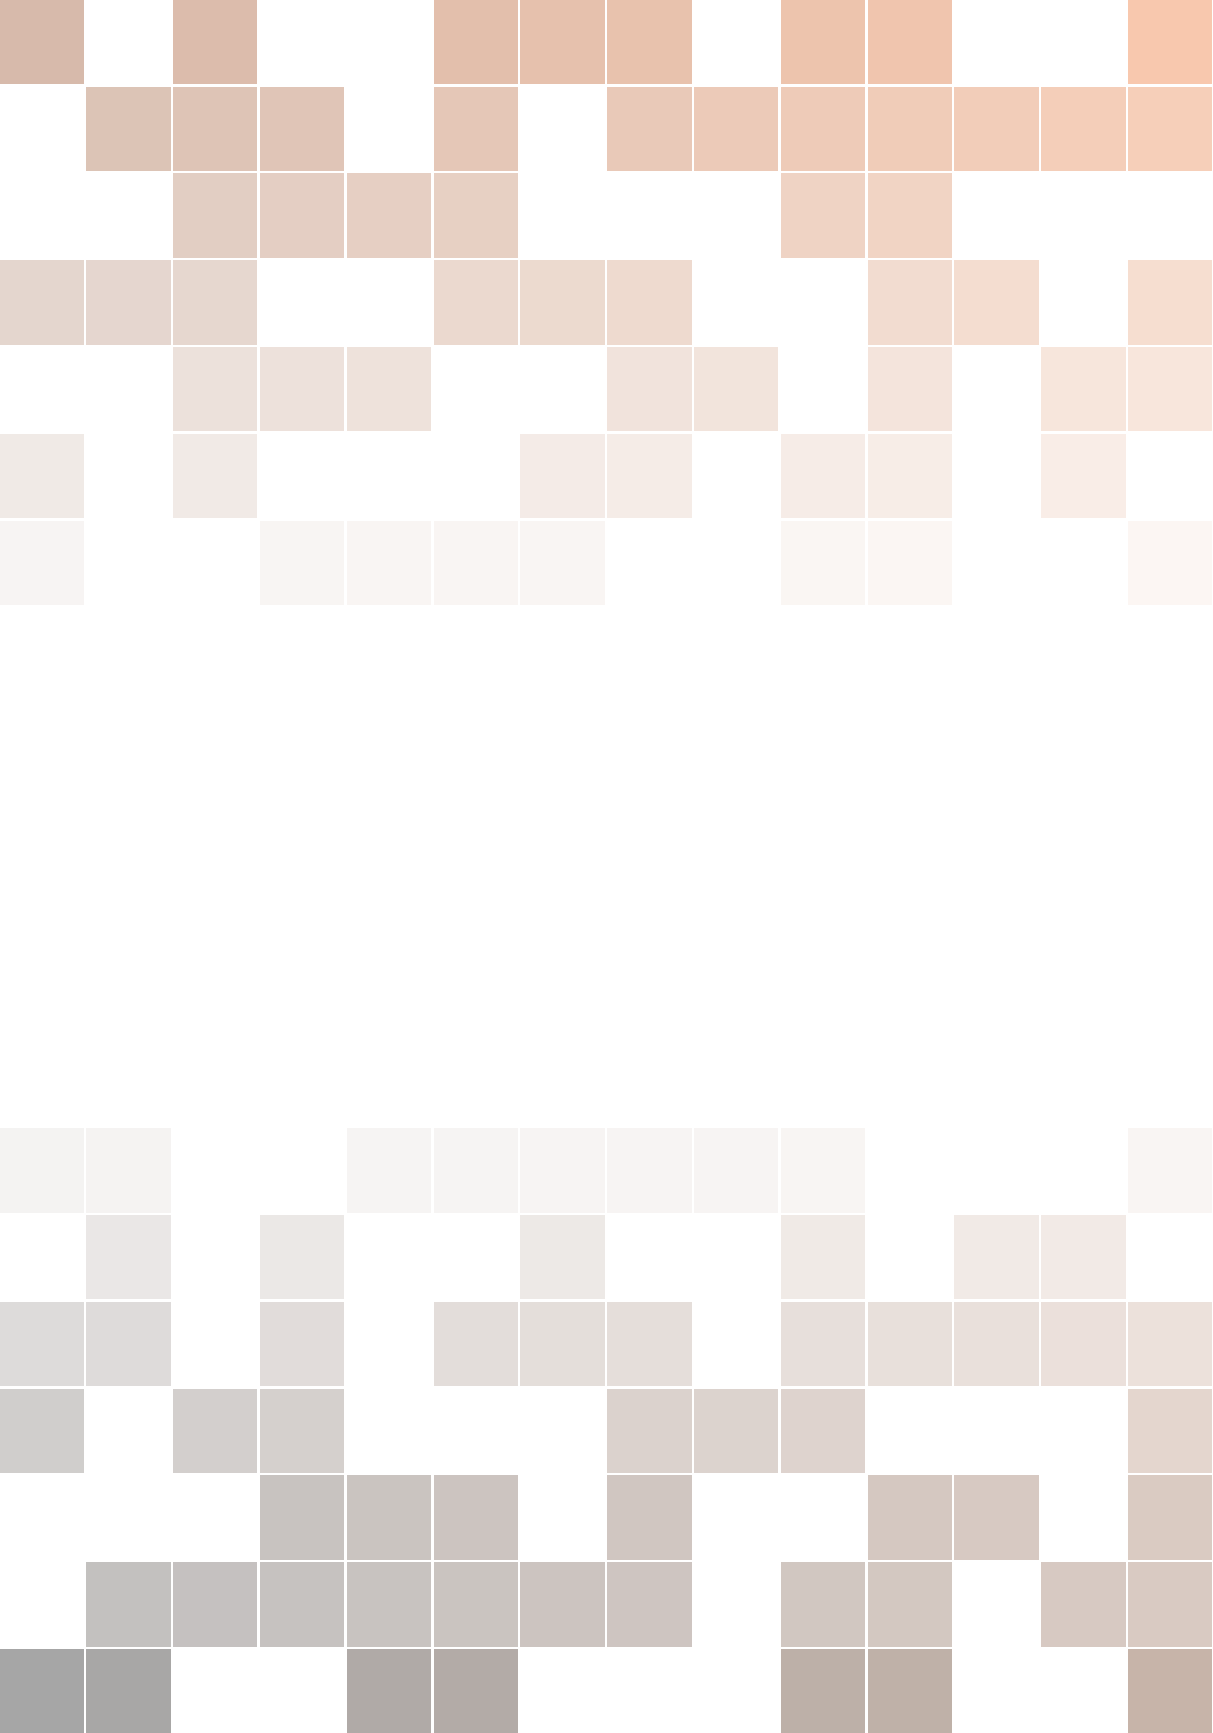
\includegraphics[width=\paperwidth]{background.pdf}};
\draw (current page.center) node [fill=ocre!30!white,fill opacity=0.6,text opacity=1,inner sep=1cm]{\Huge\centering\bfseries\sffamily\parbox[c][][t]{\paperwidth}{\centering Computational Fluid Dynamics\\[15pt] % Book title
{\Large An Open Source Approach}\\[20pt] % Subtitle
{\huge Dr. Brian C. Vermeire}}}; % Author name
\end{tikzpicture}
\vfill
\endgroup

%----------------------------------------------------------------------------------------
%	COPYRIGHT PAGE
%----------------------------------------------------------------------------------------

\newpage
~\vfill
\thispagestyle{empty}

\noindent Copyright \copyright\ 2019 Brian C. Vermeire\\ % Copyright notice

\noindent \textsc{Published by Concordia University}\\ % Publisher

\noindent \textsc{book-website.com}\\ % URL

\noindent Licensed under the Creative Commons Attribution-NonCommercial 3.0 Unported License (the ``License''). You may not use this file except in compliance with the License. You may obtain a copy of the License at \url{http://creativecommons.org/licenses/by-nc/3.0}. Unless required by applicable law or agreed to in writing, software distributed under the License is distributed on an \textsc{``as is'' basis, without warranties or conditions of any kind}, either express or implied. See the License for the specific language governing permissions and limitations under the License.\\ % License information, replace this with your own license (if any)

\noindent \textit{First printing, March 2019} % Printing/edition date

%----------------------------------------------------------------------------------------
%	TABLE OF CONTENTS
%----------------------------------------------------------------------------------------

%\usechapterimagefalse % If you don't want to include a chapter image, use this to toggle images off - it can be enabled later with \usechapterimagetrue

\chapterimage{chapter_head_1.pdf} % Table of contents heading image

\pagestyle{empty} % Disable headers and footers for the following pages

\tableofcontents % Print the table of contents itself

\cleardoublepage % Forces the first chapter to start on an odd page so it's on the right side of the book

\pagestyle{fancy} % Enable headers and footers again

%----------------------------------------------------------------------------------------
%	PART 1: Introduction
%----------------------------------------------------------------------------------------

\part{Part 1: Introduction}

\chapterimage{chapter_head_2.pdf} % Chapter heading image

\chapter{Motivation}

\section{Theory}\index{Theory}

\section{Experiments}\index{Experiments}

\section{Simulation}\index{Simulation}

\section{Digital Computing}\index{Digital Computing}

\chapter{Basic Steps}

\section{Physical Insight}\index{Physical Insight}

\section{Physical Laws}\index{Governing Physical Laws}

\section{Discretization}\index{Discretization}

\section{Programming}\index{Programming}

\section{Solving}\index{Solving}

\section{Post-Processing}\index{Post-Processing}

\chapter{Sources of Error}

%----------------------------------------------------------------------------------------
%	PART 2: Conservation Laws
%----------------------------------------------------------------------------------------

\part{Part 2: Physics}

\chapterimage{chapter_head_2.pdf} % Chapter heading image

\chapter{Conservation Laws}
Some of the most powerful tools in classical mechanics, including fluid mechanics, are conservation laws. Arising from the profound physical insights of Newton, Leibniz, and others, these laws ensure that the total amount of certain physical quantities within a volume are conserved. For example, conservation of mass ensures that the total mass of a system remains constant, conservation of momentum ensures that the total momentum of a system remains constant, and conservation of energy ensures that the total energy of a system remains constant. That is, given an isolated physical system, the total mass, momentum, and energy should remain constant and, conversely, for an open system the change in mass, momentum, and energy is equal to the amount that enters/leaves the system across its boundaries.

While these concepts can be applied by a high-school student for simple systems, such as elastic/inelastic collisions between partciles, their application to fluid mechanics is less trivial. Nevertheless, the fundamental concepts of conservation of mass, momentum, and energy still apply to fluids just as well as they do to individual particles, it is only the mathematics that becomes more complex. It is expected that students reading this book have already taken an undergraduate course in fluid mechanics and are familiar with conservation laws. Nevertheless, this chapter reviews these concepts for completeness, and to establish the notation used in the rest of the book.

\section{Reynolds Transport Theorem}\index{Reynolds Transport Theorem}
Before tackling conservation of mass, momentum, and energy in their entirety, we will first consider an arbitrary conserved {\it extensive} quantity $U_{System} = U_{System}(t)$ of a moving system of fluid, which has a related quantity per unit volume $u = u(\vec{x},t)$, where $\vec{x}$ and $t$ are the spatial coordinate and time, respectively. For example, if the extensive property is mass, than the volumetric property is mass per unit volume, or density. We start by imagining a stationary control volume (CV), denoted by $\Omega$, that is the same shape as the fluid system at some time $t$. We also denote the surface of this volume by $S$ and the outward pointing normal vector on this surface by $\hat{n}$. After some amount of time $dt$, we can imagine that the initial system of fluid embedded within the control volume will move to a deformed position and shape at $t + dt$, while the control volume remains fixed by definition. In this manner the fluid contained by the system will be equal to that of the control volume plus any incoming or outgoing fluid due to the motion of the system system boundaries as it travels with the flow.

Looking at Figure \ref{}, there are two ways that $U_{System}$ will change with time. Either via a change of $U_{CV}$ within the control volume it overlaps with, or by some amount of the conserved quantity crossing the boundary of the system as it moves. We start by getting the total amount within the control volume $U_{CV}(t)$ by simply adding up, or integrating, $u$ over it. This can be written as
\begin{equation}
	\label{eqn:totalcons}
	U_{CV}(t) = \int_\Omega u d\vec{x},
\end{equation}
noticing that the dependence on space is lost after integration. The time derivative of this is associated with the rate of change of the conserved variable within the control volume itself
\begin{equation}
	\label{eqn:totalcons}
	\frac{dU_{CV}}{dt} = \frac{d}{dt}\int_\Omega u d\vec{x}.
\end{equation}
The second term to be addressed is the change in $U_{System}$ due to its moving boundaries.

As noted previously, the second way for $U_{System}$ to change with time is by fluid crossing the surface $S$ as the fluid system moves to $t+dt$. In order for fluid to cross the surface it must be moving {\it normal} to it, otherwise it will just move along the surface and not enter the control volume. Hence, we can get the velocity component normal to the surface at any point via the normal vector. Then we can get the total amount of $u$ crossing the surface $S$ by adding up, or integrating, the normal flux at every point on the surface
\begin{equation}
	\label{eqn:totalflux}
	F(t) = \oint_S u (\vec{v} \cdot \hat{n}) ds,
\end{equation}
where $F = F(t)$ is the total rate the conserved quantity $U$ enters/leaves the control volume across the surface.

To create our conservation law we combine the concepts in Equations \ref{eqn:totalcons} and \ref{eqn:totalflux}. We note that the rate of change of the total amount of the conserved variable within the system $U_{System}$ is equal to the rate at which the conserved variable changes within the control volume and the rate it enters/leaves across the surface of the system as it moves. Mathematically this can be written as
\begin{equation}
	\frac{dU_{System}}{dt} = \frac{d}{dt}\int_\Omega u d\vec{x} + \oint_S u (\vec{v} \cdot \hat{n}) ds,
\end{equation}
noting that the positive in front of the surface term is due to our normal vector being outward pointing. Known as Reynolds Transport Theorem, this will be the foundation for deriving our conservation of mass, momentum, and energy equations for fluid flows.

\chapter{The Navier Stokes Equations}

\section{Integral Form}\index{Integral Form}
\subsection{Conservation of Mass}
When considering the mass $m = m(t)$ of our system, the mass per unit volume is the density, denoted by $\rho = \rho(\vec{x},t)$. Since the boundaries of our system move with the fluid flow, no mass can enter or leave. Hence, any mass initially within the system is confined therein and the time rate of change of $m$ is zero. Hence,
\begin{equation}
	\frac{dm}{dt} = \frac{d}{dt}\int_\Omega \rho d\vec{x} + \oint_S \rho \vec{v} \cdot \hat{n} ds = 0,
\end{equation}
and conservation of mass can be written as
\begin{eqBox}
\begin{equation}
	\frac{d}{dt}\int_\Omega \rho d\vec{x} + \oint_S \rho \vec{v} \cdot \hat{n} ds = 0.
\end{equation}
\end{eqBox}

\subsection{Conservation of Momentum}
From Newton's second-law we know that the time rate of change of the total momentum of the system is equal to the sum of all forces acting on it. Hence
\begin{equation}
	\sum \vec{F} = \frac{d(m \vec{v})}{dt},
\end{equation}
where the product $m \vec{v}$ is the total momentum of the system. Noting that the momentum per unit volume is $\rho \vec{v}$, and using Reynolds transport theorem we obtain
\begin{equation}
	 \frac{d}{dt}\int_\Omega \rho \vec{v} d\vec{x} + \oint_S \rho \vec{v} (\vec{v} \cdot \hat{n}) ds = \sum \vec{F},
\end{equation}
which requires knowledge of the forces that will act on the system at any given time, which can be split into surface and body terms. In the current context, only surface terms are considered and body terms, such as gravitational forces, are neglected.

The first of the surface forces is due to the pressure surrounding the system. Since pressure acts normal to a surface, the total pressure force $\vec{F_P}$ can be obtained via integration along the surface. Hence,
\begin{equation}
	\vec{F_P} = \oint_S -p\hat{n} ds,
\end{equation}
where $p$ is the pressure and the negative is included since pressure exerts a force inwards, but our normal vector is defined as outwards. The second set of surface terms is due to the effects of viscosity. To account for these we introduce the Cauchy stress tensor $\tau$, which for Newtonian fluids is
\begin{equation}
	\tau = \mu \left(\nabla \vec{v} + \left(\nabla \vec{v} \right)^T \right) - \frac{2}{3} \mu \left(\nabla \cdot \vec{v} \right) \mathbf{I},
\end{equation}
where $\mu$ is the dynamic viscosity and $\mathbf{I}$ is an identity matrix. Whereas pressure acts normal to the control volume surface, viscous effects act parallel to it. Hence, the total viscous force $\vec{F_v}$ can be obtained via integration
\begin{equation}
	\vec{F_v} = \oint_S \tau \cdot \hat{n} ds.
\end{equation}
With the inviscid and forces determined, conservation of momentum can be written as
\begin{equation}
	 \frac{d}{dt}\int_\Omega \rho \vec{v} d\vec{x} + \oint_S \rho \vec{v} (\vec{v} \cdot \hat{n}) ds = \oint_S -P\hat{n} ds + \oint_S \tau \cdot \hat{n} ds,
\end{equation}
which is commonly written by grouping all of the surface integral terms
\begin{eqBox}
\begin{equation}
	 \frac{d}{dt}\int_\Omega \rho \vec{v} d\vec{x} + \oint_S \left[ \rho \vec{v} \oplus \vec{v} - \sigma \right]\cdot \hat{n} ds =  0,
\end{equation}
\end{eqBox}
where
\begin{equation}
	\sigma = -p \mathbf{I} + \tau.
\end{equation}

\subsection{Conservation of Energy}
From conservation of energy, the rate of change of energy within the system is equal to the rate of heat added to the system less the rate work done by the system on its surroundings. Hence,
\begin{equation}
	\frac{dE}{dT} = \frac{dQ}{dT} - \frac{dW}{dT},
\end{equation}
where $E$ is the energy in the system, $Q$ is heat, and $W$ is work. In this case the energy per unit volume is $\rho e$ where 
\begin{equation}
e = c_v T + \frac{1}{2} \vec{v} \cdot \vec{v},
\end{equation} 
is the specific energy, $c_v$ is the specific heat at constant volume, and $T$ is the temperature. Using Reynolds transport theorem we have
\begin{equation}
\frac{d}{dt}\int_\Omega \rho e d\vec{x} + \oint_S \rho e (\vec{v} \cdot \hat{n}) ds = \frac{dQ}{dT} - \frac{dW}{dT}.
\end{equation}

Since body forces have been neglected, the work done by the system on its surroundings is due to only surface forces. The work done by pressure $\dot{W}_p$ is due to the product of the pressure force, which acts normal to the boundary, and the velocity of the boundary in the normal direction. Hence,
\begin{equation}
	\dot{W}_p = \oint_S p(\vec{v} \cdot \hat{n}) ds.
\end{equation}
Similarly, the work done by viscous forces, $\dot{W}_v$, is due to the product of the viscous stresses and the velocity on the surface. Hence, 
\begin{equation}
	\dot{W}_v = -\oint_S \tau \cdot \vec{v} ds.
\end{equation}
In the above equations note that, by convention, work is defined as from the system to the surroundings.

The second way that energy can be transferred to the system across the surfaces is thermal diffusion via conduction, denoted by $\dot{Q}$. From Fourier's law the heat diffused at any point in the fluid is
\begin{equation}
	\vec{q} = -k \nabla T,
\end{equation}
where $k$ is the thermal conductivity of the fluid. Again, only the component of heat that is diffused normal to the surface of the control volume will actually enter it. Hence, the heat added to the system is
\begin{equation}
	\dot{Q} = \oint_S k \nabla T \cdot \hat{n} ds,
\end{equation}
again noting that heat transfer is defined as from the surroundings to the system.

From the work and heat transfer terms we can now write an expression for conservation of energy
\begin{equation}
\frac{d}{dt}\int_\Omega \rho e d\vec{x} + \oint_S \rho e (\vec{v} \cdot \hat{n}) ds = \oint_S k \nabla T \cdot \hat{n} ds - \oint_S p(\vec{v} \cdot \hat{n}) ds + \oint_S (\tau \cdot \vec{v})\cdot \hat{n} ds.
\end{equation}
Similar to the momentum equation, this is often written more compactly as
\begin{eqBox}
\begin{equation}
\frac{d}{dt}\int_\Omega \rho e d\vec{x} + \oint_S \left[ \rho e \vec{v} + p\vec{v} - \tau \cdot \vec{v} - k \nabla T \right] \cdot \hat{n} ds = 0.
\end{equation}
\end{eqBox}

\subsection{Compact Integral Form}
One might notice that the conservation of mass, momentum, and energy equations derived in the previous sections all have a similar form. They include a time derivative of the conserved variable integrated over the control volume, and a surface integral term of fluxes across the control volume surface. Commonly these equations are compacted into a vector of conserved quantities
\begin{align}
	\vec{w} &= \begin{bmatrix}
		\rho \\
	    \rho \vec{v} \\
	    \rho e
	\end{bmatrix},
\end{align}
a vector of inviscid fluxes
\begin{align}
	\vec{F}_{inv} &= \begin{bmatrix}
		\rho \vec{v} \\
	    \rho \vec{v} \oplus \vec{v} + p \mathbf{I} \\
	    \rho e \vec{v} + p\vec{v}
	\end{bmatrix},
\end{align}
and viscous fluxes
\begin{align}
	\vec{F}_{vis} &= \begin{bmatrix}
		0 \\
	    -\tau \\
	    -\tau \cdot \vec{v} - \vec{q}
	\end{bmatrix}.
\end{align}
This allows the integral form of the Navier-Stokes equations to be written compactly as
\begin{eqBox}
\begin{equation}
\label{eqn:compactintegral}
\frac{d}{dt}\int_\Omega \vec{w} d\vec{x} + \oint_S \left[\vec{F}_{inv} - \vec{F}_{vis}\right] \cdot \hat{n} ds = 0.
\end{equation}
\end{eqBox}


\section{Divergence Form}\index{Divergence Form}
Looking back at the previous section, we note that Equation \ref{eqn:totalcons} is a general conservation law for a finite control volume. In some contexts, specifically when using the finite-volume method that will be introduced later, this {\it integral form} of the governing equations is used. However, other approaches in CFD use a nearly equivalent {\it divergence form} of Equation \ref{eqn:totalcons}. To derive this form we rely on the divergence theorem, also known as Gauss theorem.
\begin{theorem}[Divergence Theorem]
The divergence theorem states that integrals of the following form are equivalent for a continuously differentiable vector field $\vec{F}$
\begin{align}
\int_\Omega \nabla \cdot \vec{F} d\vec{x} = \oint_S \vec{F} \cdot \hat{n} ds,
\end{align}
which allows us to transform volume integrals into surface integrals, or the reverse.
\end{theorem}

\subsection{Conservation of Mass}
Starting from the integral form of conservation of mass and applying the divergence theorem to the surface term we obtain
\begin{equation}
	\frac{d}{dt}\int_\Omega \rho d\vec{x} + \int_\Omega \nabla \cdot (\rho \vec{v}) d\vec{x} = 0.
\end{equation}
Since integration and differentiation commute, we can bring the time derivative inside of the first integral
\begin{equation}
	\int_\Omega \frac{\partial \rho}{\partial t} d\vec{x} + \int_\Omega \nabla \cdot (\rho \vec{v}) d\vec{x} = 0.
\end{equation}
and noticing that the bounds of both integrals are the same
\begin{equation}
	\int_\Omega \left( \frac{\partial \rho}{\partial t} + \nabla \cdot (\rho \vec{v}) \right) d\vec{x} = 0.
\end{equation}
In order for this equation to be valid, other than in trivial cases, we require that the integrand be identically zero. Hence, conservation of mass in divergence form can be written as
\begin{eqBox}
\begin{equation}
	\frac{\partial \rho}{\partial t} + \nabla \cdot (\rho \vec{v}) = 0.
\end{equation}
\end{eqBox}
It is interesting to note that we have effectively converted a problem involving surface and volume integrals, into a differential form that requires computing derivatives.

\begin{remark}
A subtle difference between the two forms of conservation laws is that the integral form applies to control volumes and the divergence form applies at points. This will become important in choosing what form to use for CFD, and will be explored later.
\end{remark}

\subsection{Conservation of Momentum}
Applying the same sets of operations to the integral form of the momentum equation we can obtain its divergence form
\begin{eqBox}
\begin{equation}
	 \frac{\partial \rho \vec{v}}{\partial t} + \nabla \cdot \left[ \rho \vec{v} \oplus \vec{v} - \sigma \right] =  0.
\end{equation}
\end{eqBox}

\subsection{Conservation of Energy}
Applying the same sets of operations to the integral form of the energy equation we can obtain its divergence form
\begin{eqBox}
\begin{equation}
\frac{\partial \rho e}{\partial t} + \nabla \cdot \left[ \rho e \vec{v} + p\vec{v} - \tau \cdot \vec{v} - k \nabla T \right] = 0.
\end{equation}
\end{eqBox}

\subsection{Compact Divergence Form}
Considering the compact integral form given in Equation \ref{eqn:compactintegral}, we notice that the divergence theorem can also be applied. Hence, a compact differential form of the Navier-Stokes equations can be obtained
\begin{eqBox}
\begin{equation}
\frac{\partial \vec{w}}{\partial t} + \nabla \cdot \left[\vec{F}_{inv} - \vec{F}_{vis}\right] = 0.
\end{equation}
\end{eqBox}

\chapter{Simplified Systems}

One might notice that the Navier-Stokes equations derived in the previous chapter are a complex system of coupled non-linear partial differential equations. This is not something that sounds particularly easy to solve! Hence, in CFD we often consider {\it simplified} systems of equations first, neglecting or decoupling some of the physical mechanisms that are involved in the full Navier-Stokes equations. This allows us to play with different ideas quickly and with relative ease. Then, once we understand of how to solve different parts of these simplified equations, we will combine these ideas later to solve the full Navier-Stokes equations. 

\section{Euler Equations}\index{Euler Equations}
The Euler equations, although they were actually derived prior Navier-Stokes, can be obtained by simply neglecting viscous effects. Hence, we can ignore physical viscosity and thermal diffusion. While historically the Euler equations were the state-of-the-art in CFD, their lack of viscosity means they are unsuitable for predicting boundary layers. Nevertheless, they are still useful for predicting many flow phenomena, such as shockwaves.

In integral form the Euler equations are
\begin{eqBox}
\begin{equation}
	 \frac{d}{dt}\int_\Omega \rho d\vec{x} + \oint_S \rho \vec{v} \cdot \hat{n} ds = 0,
\end{equation}
\begin{equation}
	\frac{d}{dt}\int_\Omega \rho \vec{v} d\vec{x} + \oint_S \left[ \rho \vec{v} \oplus \vec{v} + p \mathbf{I} \right]\cdot \hat{n} ds =  0,
\end{equation}
\begin{equation}
	\frac{d}{dt}\int_\Omega \rho e d\vec{x} + \oint_S \left[ \rho e \vec{v} + p\vec{v} \right] \cdot \hat{n} ds = 0,
\end{equation}
\end{eqBox}
for conservation of mass, momentum, and energy, respectively. Similarly, in divergence form the Euler equations are
\begin{eqBox}
\begin{equation}
	 \frac{\partial \rho}{\partial t} + \nabla \cdot (\rho \vec{v}) = 0,
\end{equation}
\begin{equation}
	\frac{\partial \rho \vec{v}}{\partial t} + \nabla \cdot \left[ \rho \vec{v} \oplus \vec{v} + p \mathbf{I} \right] =  0,
\end{equation}
\begin{equation}
	\frac{\partial \rho e}{\partial t} + \nabla \cdot \left[ \rho e \vec{v} + p\vec{v} \right] = 0,
\end{equation}
\end{eqBox}
for conservation of mass, momentum, and energy.

\section{Linear Advection}\index{Linear Advection}
Even if we consider the Euler equations, we notice that they are still relatively complex and difficult to solve. In what follows we will use a set of thought experiments to generate a set of three much simpler equations that will be a starting point for our initial exploration of CFD. To start, we will derive the so-called linear advection equation. We begin our thought experiment by considering a fluid flow that has uniform velocity throughout the domain. Furthermore, we will decouple conservation of mass from the other two conservation laws. 

Now we can imagine that our fluid flow, with constant velocity everywhere such that $\vec{v}(\vec{x},t) = \vec{\alpha}$, has some blob of fluid that is dense relative to the rest of the fluid around it. For example, it could be slightly colder, increasing its density. What should happen to this blob of fluid over time? Well since the fluid is all moving at the same velocity $\vec{\alpha}$ we would expect the blob of dense fluid to simply move along with the rest of the flow and, hence, the blob should move at velocity $\vec{\alpha}$.

Mathematically this yields the following integral and differential forms for the linear advection equation by using conservation of mass and replacing the velocity by a constant velocity field $\vec{\alpha}$ and the density by a general scalar $u$ we obtain,
\begin{eqBox}
\begin{equation}
	\frac{d}{dt}\int_\Omega u d\vec{x} + \oint_S (\vec{\alpha}u) \cdot \hat{n} ds = 0.
\end{equation}
and
\begin{equation}
	\frac{\partial u}{\partial t} + \nabla \cdot (\vec{\alpha} u) = 0.
\end{equation}
\end{eqBox}
Furthermore, if we restrict ourselves to one-dimensional problems we obtain the following integral and differential forms for linear advection
\begin{eqBox}
\begin{equation}
	\frac{d}{dt}\int_\Omega u dx + \alpha \oint_S u \cdot \hat{n} ds = 0,
\end{equation}
and
\begin{equation}
	\frac{\partial u}{\partial t} +  \alpha \frac{\partial u}{\partial x} = 0.
\end{equation}
\end{eqBox}

\section{Burgers Equation}\index{Burgers Equation}
Our second simplified system, known as Burgers equation, is useful as a simplified model for compressible flow features such as shocks and expansion fans. To derive Burgers equation we start with the momentum equation, decoupled from conservation of mass and conservation of energy. Then, neglecting the effects of viscosity and pressure, we replace the momentum with an arbitrary conserved variable $u$, and restrict ourselves to one physical dimension. 

This yields the following integral and differential forms of the Burgers equation
\begin{eqBox}
\begin{equation}
	 \frac{d}{dt}\int_\Omega u dx + \frac{1}{2}\oint_S u^2 \cdot \hat{n} ds =  0,
\end{equation}
and
\begin{equation}
	\frac{\partial u}{\partial t} +  \frac{1}{2} \frac{\partial u^2}{\partial x} = 0.
\end{equation}
\end{eqBox}
noting that the factor of one half is added to the spatial term by convention.

If we consider the divergence form of Burgers' equation, applying chain rule to the spatial derivative operator yields
\begin{equation}
	\frac{\partial u}{\partial t} +  u \frac{\partial u}{\partial x} = 0.
\end{equation}
We note that this looks remarkably similar to the divergence form of the linear advection equation, also in one dimension. However, the advection velocity $\alpha$, which appears infront of the spatial derivative for linear advection, has instead been replaced by $u$, the value of the solution. Hence, Burgers equation has similar behaviour to linear advection, except the velocity at any point in space is {\it equal} to the value of the solution at that point, rather than being a constant value throughout the domain.

\section{Linear Diffusion}\index{Linear Diffusion}
Our third and final simplified equation, known as linear diffusion, starts again from a simple thought experiment. First, we will consider only the energy equation decoupled from conservation of mass and momentum. We will now imagine that we have a stationary fluid with zero velocity everywhere in the domain. Similar to linear advection, we will consider a flow with some blob of fluid with more energy than the fluid around it. Since all of the fluid is stationary, this extra energy must come in the form of heat. As time goes on, we would expect that this local region of hot fluid would diffuse some of its heat over time to the cold fluid that is adjacent to it. Hence, over time an initially concentrated blob of heat would spread out, until eventually all of the fluid is at the same temperature.

Mathematically, the equation describing this can be obtained by taking $\alpha = k/{\rho c_v}$ as a constant scalar and replacing $e$ with a generic scalar $u$. We can then rewrite the energy equation in multiple dimensions as
\begin{eqBox}
\begin{equation}
\frac{d}{dt}\int_\Omega u d\vec{x} + \oint_S \left[ - \alpha \nabla u \right] \cdot \hat{n} ds = 0.
\end{equation}
and
\begin{equation}
\frac{\partial u}{\partial t} - \nabla \cdot (\alpha \nabla u) = 0,
\end{equation}
\end{eqBox}
in integral and divergence form, respectively. Furthermore, if we restrict ourselves to one dimension we obtain
\begin{eqBox}
\begin{equation}
\frac{d}{dt}\int_\Omega u dx + \oint_S \left[ - \alpha  \frac{\partial u}{x} \right] \cdot \hat{n} ds = 0.
\end{equation}
and
\begin{equation}
\frac{\partial u}{\partial t} - \alpha \frac{\partial^2 u}{\partial x^2} = 0.
\end{equation}
\end{eqBox}
At this point it is worth noting that the form of the linear diffusion equation is similar to the linear advection equation, except we are taking the second derivative rather than the first.

\chapter{Turbulence}
\section{Turbulence Theory}
\subsection{Introduction to Chaos}
\subsection{Chaos and Navier-Stokes}
\subsection{The Energy Cascade}
\section{Reynolds Averaging}
\subsection{The Reynolds Averaged Navier-Stokes Equations}
\subsection{The Reynolds Stresses}
\section{Turbulence Modelling}
\subsection{The Boussinesq Hypothesis}
\subsection{The Mixing Length Model}
\subsection{The Spalart-Allmaras Model}
\subsection{The k-$\epsilon$ Model}
\subsection{The k-$\omega$ Model}
\subsection{Summary of Turbulence Models}

\chapter{Boundary Conditions}
\section{Wall Boundaries}
\subsection{Wall-Bounded Turbulence}
\subsection{Boundary Conditions}
\subsection{Wall Modelling}
\section{Farfield Boundaries}
\subsection{Non-Reflecting Boundaries}

%----------------------------------------------------------------------------------------
%	PART 3: Finite Difference Methods
%----------------------------------------------------------------------------------------

\part{Part 3: Finite Difference Methods}

\chapterimage{chapter_head_2.pdf} % Chapter heading image

\chapter{Taylor-Series}

\section{Grid Spacing}\index{Grid Spacing}

\section{Number of Terms}\index{Number of Terms}

\chapter{Finite Difference Methods}

\chapter{Examples}

\section{Linear Advection}\index{Linear Advection}

\section{Burgers Equation}\index{Burgers Equation}

\section{Linear Diffusion}\index{Linear Diffusion}

%----------------------------------------------------------------------------------------
%	PART 4: Finite Volume Methods
%----------------------------------------------------------------------------------------

\part{Part 4: Finite Volume Methods}

\chapterimage{chapter_head_2.pdf} % Chapter heading image

\chapter{Volume Averaging}

%----------------------------------------------------------------------------------------
%	BIBLIOGRAPHY
%----------------------------------------------------------------------------------------

\chapter*{Bibliography}
\addcontentsline{toc}{chapter}{\textcolor{ocre}{Bibliography}} % Add a Bibliography heading to the table of contents

%------------------------------------------------

\section*{Articles}
\addcontentsline{toc}{section}{Articles}
\printbibliography[heading=bibempty,type=article]

%------------------------------------------------

\section*{Books}
\addcontentsline{toc}{section}{Books}
\printbibliography[heading=bibempty,type=book]

%----------------------------------------------------------------------------------------
%	INDEX
%----------------------------------------------------------------------------------------

\cleardoublepage % Make sure the index starts on an odd (right side) page
\phantomsection
\setlength{\columnsep}{0.75cm} % Space between the 2 columns of the index
\addcontentsline{toc}{chapter}{\textcolor{ocre}{Index}} % Add an Index heading to the table of contents
\printindex % Output the index

%----------------------------------------------------------------------------------------

\end{document}
